%==============================================================================
\chapter{Large-Scale RDF Dataset Statistics}
\label{chapter:dist_lod_stats}
%==============================================================================

Over the last two decades, the Semantic Web has grown from a mere idea for modeling data in the web, into an established field of study driven by a wide range of standards and protocols for data consumption, publication, and exchange on the Web.
For the record, today we count more than 10,000 datasets openly available online using Semantic Web standards~\furl{http://lodstats.aksw.org/}.
Thanks to such standards, large datasets became machine-readable~\cite{rw2014}.
Nevertheless, many applications such as data integration, search, and interlinking may not take full advantage of the data without having \textit{a priori} statistical information about its internal structure and coverage. 
\gls{RDF} dataset statistics can be beneficial in many ways, for example: 1) Vocabulary reuse (suggesting frequently used similar vocabulary terms in other datasets during dataset creation), 2) Quality analysis (analysis of incoming and outcoming links in \gls{RDF} datasets to establish hubs similar to what PageRank has achieved in the traditional web), 3) Coverage analysis (verifying whether frequent dataset properties cover all similar entities and other related tasks), 4) privacy analysis (checking whether property combinations may allow to uniquely identify persons in a dataset) and 5) link target analysis (finding datasets with similar characteristics, e.g.~similar frequent properties) for interlinking candidates.

A number of solutions have been conceived to offer users such statistics about \gls{RDF} vocabularies~\cite{vandenbussche2015linked} and datasets~\cite{conf/dexaw/LangeggerW09,ermilov-2013-kesw}.
However, those efforts showed severe deficiencies in terms of performance when the dataset size goes beyond the main memory size of a single machine.
This limits their capabilities to medium-sized datasets only, which paralyzes the role of applications in embracing the increasing volumes of the available datasets.

As the memory limitation was the main shortcoming in the existing works, we investigated parallel approaches that distribute the workload among several separate memories.
One solution that gained traction over the past years is the concept of \gls{RDD}, initially suggested at~\cite{zaharia2012resilient}, which are in-memory data structures. 
Using \gls{RDD}s, we are able to perform operations on the whole dataset stored in a significantly enlarged distributed memory.

Apache Spark~\furl{http://spark.apache.org} is an implementation of the concept of \gls{RDD}s.
It allows performing coarse-grained operations over voluminous datasets in a distributed manner in parallel.
It extends earlier efforts in the area such as Hadoop MapReduce.

In this chapter we address the following research question:
\begin{tcolorbox}
\textbf{RQ1}: How can we efficiently explore the structure of large-scale \gls{RDF} datasets?
\end{tcolorbox}

Contributions of this chapter are summarize as follows:
\begin{itemize}
    \item We propose an algorithm for computing \gls{RDF} dataset statistics and implement it using an efficient framework for large-scale, distributed and in-memory computations: Apache Spark.
    \item We perform an analysis of the complexity of the computational steps and the data exchange between nodes in the cluster. 
    \item We evaluate our approach and demonstrate empirically its superiority over a previous centralized approach.
    \item We integrated the approach into the SANSA framework, where it is actively maintained and re-uses the community infrastructure (mailing list, issues trackers, website, etc.).
    \item An approach for triggering \gls{RDF} statistics calculation remotely simply using HTTP requests. 
    DistLODStats is built as a plugin into the larger SANSA framework and makes use of Apache Livy, a novel lightweight solution for interacting with the Spark cluster via a REST Interface.
\end{itemize}

This chapter is based on the following publications (\cite{sejdiu-2018-dist-lod-stats-iswc,sejdiu-2018-statisfy-iswc-poster}):
\begin{itemize}
    \item \textbf{Gezim Sejdiu}; Ivan Ermilov; Jens Lehmann; and Mohamed Nadjib-Mami, “\href{http://jens-lehmann.org/files/2018/iswc_distlodstats.pdf}{DistLODStats: Distributed Computation of RDF Dataset Statistics},” in Proceedings of 17th International Semantic Web Conference (ISWC), 2018.

    \item \textbf{Gezim Sejdiu}; Ivan Ermilov; Jens Lehmann; and Mohamed-Nadjib Mami, “\href{http://jens-lehmann.org/files/2018/iswc_statisfy_pd.pdf}{STATisfy Me: What are my Stats?},” in Proceedings of 17th International Semantic Web Conference (ISWC), Poster \& Demos, 2018.
\end{itemize}

The remainder of this chapter is organized as follows: 
Our approach for the computation of \gls{RDF} dataset statistics is detailed in Section~\ref{sec:approach}.
An analysis of the complexity of the computational steps and the data exchange between nodes is conducted in Subsection~\ref{subsection:complexAnalys} to assess the complexity of each statistical criterion.
The evaluation of the approach is elaborated in Subsection~\ref{sec:evaluation}.
STATisfy, a component for triggering \gls{RDF} statistics calculation remotely by using HTTP request has been described in Section~\ref{sec:distlodstats-statisfy}.
Finally, we summarize our work in Section~\ref{sec:distlodstats-summary}.

\section{A Scalable Distributed Approach for Computation of RDF Dataset Statistics}
\label{sec:approach}
We adopted the 32 statistical criteria proposed in~\cite{demter-2012-ekaw}.
In contrast to~\cite{demter-2012-ekaw}, we perform the computation in a large-scale distributed environment using Spark and the concept of \gls{RDD}s.
Instead of processing the input \gls{RDF} dataset directly, this approach requires the conversion to an \gls{RDD} that is composed of three elements: \emph{Subject}, \emph{Property} and \emph{Object}.
We name such an \gls{RDD} a \emph{main dataset}.

The statistical criteria proposed in \cite{demter-2012-ekaw} are formalized as a triple $(F,D,P)$ consisting of a filter condition $F$, a derived dataset $D$ and a post processing operation $P$. 
In our approach, we adapt the definition of those elements to be applicable to \gls{RDD}s.

\begin{definition}[Statistical criterion]
\label{def:statcriteria}
A statistical criterion $\mathcal{C}$ is a triple $\mathcal{C} = (F, D, P)$, where:
  
 \begin{itemize}
 \item $F$ is a \gls{SPARQL} filter condition. 
 \item $D$ is a derived dataset from the main dataset (\gls{RDD} of triples) after applying F.
 \item $P$ is a post-processing filter operating on the data structure $D$.
\end{itemize}
\end{definition}
\noindent
$F$ acts as a filter operation, which determines whether a specific criterion is matched against a triple in the \emph{main dataset}.
$D$ is the result of applying the criterion on the \emph{main dataset}.
$P$ is an operation applied to $D$ to (optionally) perform further computational steps.
If no extra computation is needed, $P$ just returns exactly the results from the intermediate dataset $D$.

\subsection{Main Dataset Data Structure}
The \emph{main dataset} is based on an \gls{RDD} data structure which is a basic building block of the Spark framework.
\gls{RDD}s are in-memory collections of records that can be operated in parallel on large clusters.
By using \gls{RDD}s, Spark abstracts away the differences of the underlying data sources.
\gls{RDD}s during their lifecycle are kept in-memory, which enables efficient reuse of \gls{RDD}s during several consequent transformations.
Spark provides fault-tolerance by keeping a lineage information (a \gls{DAG} of transformations) for each \gls{RDD}.
This way any \gls{RDD} can be reconstructed in case of node failure by tracing back the lineage.
Spark enables full control over the persistence state and partitioning of the \gls{RDD}s in the cluster.
Thus, we can further improve the computational efficiency of statistical criteria by planning a suitable storage strategy (i.e.~alternating between memory and disk).
For example, we can precisely determine which \gls{RDD}s will be reused and manage the degree of parallelism by specifying how an \gls{RDD} is partitioned across the available resources.

\begin{definition}[Basic Operations]
\label{def:basicdefination}
All the statistical criteria can be represented in our approach using the following basic operations: \textit{map}, \textit{filter}, \textit{reduce-by}, and \textit{group-by}.
These operations can be formalized as follows:
\begin{itemize}
    \item $map: I \rightarrow O$, where $I$ is an input \gls{RDD} and $O$ is an output \gls{RDD}. \textit{Map} transforms each value from an input RDD into another value, following a specified rule. %(\verb!rdd.map(f)!).
    \item $filter: I \rightarrow O$, where $I$ is an input \gls{RDD} and $O$ is an output \gls{RDD}, which contains only the elements that satisfy a condition. 
    \item $reduce: I \rightarrow O$, where $I$ is an input \gls{RDD} of key-value (K,V) pairs and $O$ is an output \gls{RDD} of (K, list(V)) pairs.
    
    \item \textit{group-by} $: (I, F) \rightarrow O$, where $I$ is an input \gls{RDD} of pairs (K, list(V)), $F$ is a grouping function (e.g., count, avg), and $O$ is an output \gls{RDD} containing the values in $list(V)$ from $I$ aggregated using the grouping function.
    
\end{itemize}
\end{definition}

\subsection{Distributed LODStats Architecture}
The computation of statistical criteria is performed as depicted in Figure~\ref{fig:RDD_Lineage}.
Our approach consists of three steps: (1) saving \gls{RDF} data in scalable storage, (2) parsing and mapping the \gls{RDF} data into the \emph{main dataset}, and (3) performing statistical criteria evaluation on the \emph{main dataset} and generating results.

\begin{figure}
\centering
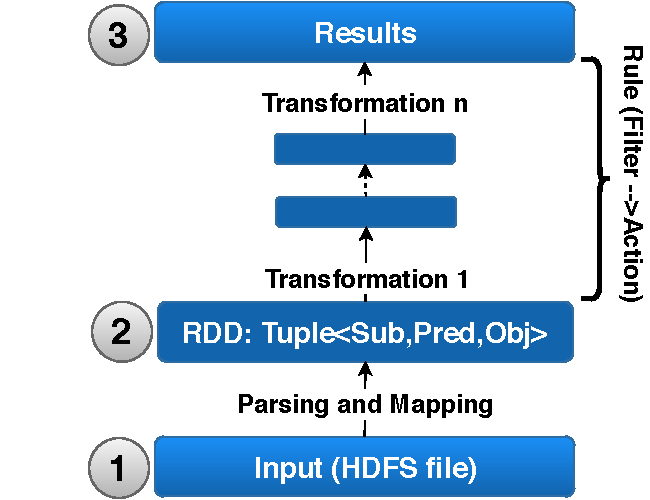
\includegraphics[width=.45\columnwidth]{images/4_distlodstats/distlodstats-rdd-lineage.pdf}
\caption{\textbf{RDD lineage of a Criterion execution}. 
It consists of three steps: (1) saving RDF data into a scalable storage, (2) parsing and mapping RDF into the main dataset (RDD of triples), and (3) performing statistical criteria evaluation on the main dataset.}
\label{fig:RDD_Lineage}
\end{figure}

\defn{Fetching the \gls{RDF} data (Step 1):} \gls{RDF} data needs first to be loaded into a large-scale storage that Spark can efficiently read from.
For this purpose, we use \gls{HDFS}~\furl{https://hadoop.apache.org/docs/r1.2.1/hdfs\_design.html}.
\gls{HDFS} is able to accommodate any type of data in its raw format, horizontally scale to an arbitrary number of nodes, and replicate data among the cluster nodes for fault tolerance.
In such a distributed environment, Spark adopts different data locality strategies to try to perform computations as close to the needed data as possible in \gls{HDFS} and thus avoid data transfer overhead.
 
\defn{Parsing and mapping \gls{RDF} into the main dataset (Step 2):} In the course of Spark execution, data is parsed into triples and loaded into an \gls{RDD} of the following format: \emph{Triple$<$Subj,Pred,Obj$>$} (by using the Spark \textit{map} transformation).

\defn{Statistical criteria evaluation (Step 3):} For each criterion, Spark generates an execution plan, which is composed of one or more of the following Spark transformations: \textit{map}, \textit{filter}, \textit{reduce} and \textit{group-by}. 

\subsection{Algorithm}
\label{sec:Algorithm}
The DistLODStats algorithm (see Algorithm~\ref{alg:DistLODStats}) constructs the \emph{main dataset} from an \gls{RDF} file (Line \ref{line:rdf2rdd}).
Afterwards, the algorithm iterates over the criteria defined inside the DistLODStats framework and evaluates them (Lines \ref{line:filter}, \ref{line:action} and \ref{line:postProc}).

To define a statistical criterion inside the DistLODStats framework, one must specify \emph{filter}, \emph{action}, and \emph{postProc} methods. 
The evaluation of the criterion then starts first by the \emph{filter} method (Line \ref{line:filter}) that is used to apply the rule filters of the criterion (Rule Filter in Table~\ref{tab:SparkRules}). 
Applied on a \emph{main dataset}, this latter will return a new \gls{RDD} with a subset of the triples.
Next, the \emph{action} method is used to apply the criterion's rule action (Rule Action in Table~\ref{tab:SparkRules}).
Applied on the filtered \gls{RDD}, this either computes statistics directly or reorganizes the \gls{RDD} so statistics can be computed in the next step.
At the end, the \emph{postProc} method is used as an optional operation to perform further statistical computations (e.g.~average after count or sort).

\begin{algorithm}
\caption{DistLODStats.}
\label{alg:DistLODStats}
\SetKwInOut{Input}{input}\SetKwInOut{Output}{output}
\Input{$RDF$: an RDF dataset,
	   $C$: a list of criterion.
      }
%\Output{...}
    \tcc{Iterate through the list of criteria}
    $RDD~\textit{mainDataset} = RDF.toRDD<Triple>()$ \label{line:rdf2rdd} \\
    %$RDD[]~results = new RDD<Triple>()$\\
    $\textit{mainDataset}.cache() $ \label{line:cache}\\
    %like here: triples = triples.cache() or triples.persist(StorageLevel.getLevel())- which can be configured by user itself (DISK/MEMORY_ONLY/DISK_AND_MEMORY,,,,).
    \ForEach{$c \in C$}{
        %\tcc{Class reflection}
        %$c \leftarrow new~instanceOf(getClassFrom(cr))$ \label{line:clssReflct}\\
        $triples \leftarrow c.filter(\textit{mainDataset})$ \label{line:filter}\\
        $triples.cache()$\label{line:cache_triples}\\
        $triples \leftarrow c.action(triples)$  \label{line:action}\\
        \If{c.hasPostProc}{
            $triples \leftarrow c.postProc(triples)$ \label{line:postProc}
        }
        %$results.add(triples)$
    }
\end{algorithm}

In our work, we make use of Spark caching techniques. 
Basically, if an \gls{RDD} is constructed from a data source e.g. file, or through a lineage of
\gls{RDD}s, and then cached, there is no need to construct the \gls{RDD} again the next time it is needed.
We have used two different approaches for caching: (1) caching the \emph{main dataset} entirely (Line~\ref{line:cache}), and (2) caching a derived \gls{RDD} after applying the criteria \emph{filter} on the \emph{main dataset} (Line~\ref{line:cache_triples}). 
In the first approach, the \gls{RDD} is constructed from the \gls{RDF} source during the first criteria computation, so the next criteria do not need to fetch it again. 
In the second approach, the \gls{RDD} resulting from executing the \emph{filter} of one criterion is cached and used by any other criterion sharing the same \textit{filter} pattern. 

 \begin{table*}
    \centering
    \begin{tabular}{>{\tiny}l>{\tiny}l|>{\tiny}l>{\tiny}l|>{\tiny}l}
      \textbf{} & 
      \textbf{Criterion} & 
      \multicolumn{2}{l|}{\textbf{\tiny Rule (Filter $\rightarrow$ Action)}} & 
      \textbf{Postproc.} \\ 
    \hline
       \refstepcounter{hdItemCounter}\thehdItemCounter\label{cr:1}  & 
      used classes & 
      \verb|p=RDF_TYPE && o.isURI()| & 
      $\rightarrow$  \verb|map(_.o)| & -- \\
    \hline
      \refstepcounter{hdItemCounter}\thehdItemCounter\label{cr:2}  & 
      class usage count & 
     \verb|p=RDF_TYPE && o.isURI()| & 
     $\rightarrow$   \verb|map(f => (f.o, 1)).reduceByKey(_ + _)| &
      \verb|take(100)| \\ 
    \hline
      \refstepcounter{hdItemCounter}\thehdItemCounter\label{cr:3}  & 
      classes defined & 
      \verb|p=RDF_TYPE && s.isURI()&&|  & 
      $\rightarrow$ \verb|map(_.s)| & --
      \\ 
      & 
      & 
      \verb/(o=RDFS_CLASS||o=OWL_CLASS)/
      &  
      & \\ 
    \hline
      \refstepcounter{hdItemCounter}\thehdItemCounter\label{cr:4}  & 
      class hierarchy & 
      \verb|p=RDFS_SUBCLASS_OF &&| & 
      $\rightarrow$ \verb|G += (?s,?o)| &  
      \verb|depth(G)| \\ 
      & 
      depth & 
      \verb|s.isIRI() && o.isIRI()| & 
      &
       \\ 
    \hline
       \refstepcounter{hdItemCounter}\thehdItemCounter\label{cr:5} & 
      property usage & 
      & 
      $\rightarrow$  \verb|map(f => (f.p, 1)).reduceByKey(_ + _)| & 
      \verb|take(100)| \\ 
    \hline
       \refstepcounter{hdItemCounter}\thehdItemCounter\label{cr:6} & 
      prop. usage per subj. & 
      & 
      $\rightarrow$ \verb|groupBy(_.s).reduceByKey(_ + _)|  & 
      \verb|count| \\
    \hline
       \refstepcounter{hdItemCounter}\thehdItemCounter\label{cr:7} & 
      prop. usage per obj. & 
      & 
      $\rightarrow$ \verb|groupBy(_.o).reduceByKey(_ + _)|  & 
      \verb|count| \\
    \hline
       \refstepcounter{hdItemCounter}\thehdItemCounter\label{cr:8} & 
      prop. distinct per subj. & 
      & 
      $\rightarrow$ \verb|groupBy(_.s).combineByKey(_ + _)|  & 
      \verb|sum/count| \\
    \hline
       \refstepcounter{hdItemCounter}\thehdItemCounter\label{cr:9} & 
      prop. distinct per obj. & 
      & 
      $\rightarrow$ \verb|groupBy(_.o).combineByKey(_ + _)|  & 
      \verb|sum/count| \\
    \hline
       \refstepcounter{hdItemCounter}\thehdItemCounter\label{cr:10} & 
      outdegree & 
      & 
      $\rightarrow$ \verb|map(f => (f.s, 1)).combineByKey(_ + _)|  & 
      \verb|sum/count| \\ 
    \hline
       \refstepcounter{hdItemCounter}\thehdItemCounter\label{cr:11} & 
      indegree & 
      & 
      $\rightarrow$ \verb|map(f => (f.o, 1)).combineByKey(_ + _)|  & 
      \verb|sum/count| \\ 
    \hline
       \refstepcounter{hdItemCounter}\thehdItemCounter\label{cr:12} & 
      property & 
     \verb|p=RDFS_SUBPROPERTY_OF &&|
      & 
      $\rightarrow$ \verb|G += (?s,?o)| &  
      \verb|depth(G)| \\ 
      & 
      hierarchy depth & 
      \verb|s.isIRI() && o.isIRI()| & 
      &
      \\ 
    \hline
       \refstepcounter{hdItemCounter}\thehdItemCounter\label{cr:13} & 
      subclass usage & 
      \verb|p=RDFS_SUBPROPERTY_OF| &
      $\rightarrow$ \verb|count()|  & 
      -- \\ 
    \hline
       \refstepcounter{hdItemCounter}\thehdItemCounter\label{cr:14} & 
      triples &  
      & 
      $\rightarrow$ \verb|count()| & 
      --\\ 
    \hline
       \refstepcounter{hdItemCounter}\thehdItemCounter\label{cr:15} & 
      entities mentioned &  
      & 
      $\rightarrow$ \verb|map(f=>(s.isURI(),p.isURI(),o.isURI())).count| 
      & --  \\
    \hline
       \refstepcounter{hdItemCounter}\thehdItemCounter\label{cr:16} & 
      distinct entities &  
      & 
      $\rightarrow$ \verb|map(f=>(s.isURI(),p.isURI(),o.isURI())).distinct| 
      & --  \\
    \hline
     \refstepcounter{hdItemCounter}\thehdItemCounter\label{cr:17} & literals &  \verb|o.isLiteral()| & $\rightarrow$ \verb|count()| & -- \\ \hline 
     \refstepcounter{hdItemCounter}\thehdItemCounter\label{cr:18} & blanks as subj. & \verb|s.isBlank()| & $\rightarrow$ \verb|count()| & -- \\ \hline 
     \refstepcounter{hdItemCounter}\thehdItemCounter\label{cr:19} & blanks as obj. & \verb|o.isBlank()| & $\rightarrow$ \verb|count()| & -- \\ \hline 
     \refstepcounter{hdItemCounter}\thehdItemCounter\label{cr:20} & datatypes & \verb|o.isLiteral()| & $\rightarrow$ \verb|map(o => (o.dataType(), 1)).reduceByKey(_ + _)| & --  \\
    \hline
       \refstepcounter{hdItemCounter}\thehdItemCounter\label{cr:21} & 
      languages & 
       \verb|o.isLiteral()| & 
       $\rightarrow$ \verb|map(o => (o.languageTag(), 1)).reduceByKey(_ + _)| 
      & -- \\
    \hline
       \refstepcounter{hdItemCounter}\thehdItemCounter\label{cr:22} & 
    %  $\diameter$ typed string & 
       average typed string &
       \verb|o.isLiteral() && obj| & 
      $\rightarrow$ \verb|count();| & 
      \verb|len/count| \\ 
      & 
      length & 
      \verb|.getDatatype()=XSD_STRING)| & 
      \verb|len+=o.length()| & 
      \\ 
    \hline
       \refstepcounter{hdItemCounter}\thehdItemCounter\label{cr:23} & 
      %$\diameter$ untyped & 
      average untyped & 
      \verb|o.isLiteral() &&| & 
      $\rightarrow$ \verb|count();| & 
      \verb|len/count| \\ 
      & 
      string length & 
      \verb|o.getDatatype().isEmpty()| & 
      \verb|len+=o.length()|& 
      \\ 
    \hline
     \refstepcounter{hdItemCounter}\thehdItemCounter\label{cr:24} & typed subject & \verb|p=RDF_TYPE| & $\rightarrow$ \verb|count()| & -- \\ \hline
     \refstepcounter{hdItemCounter}\thehdItemCounter\label{cr:25} & labeled subject & \verb|p=RDFS_LABEL| &  $\rightarrow$ \verb|count()| & -- \\ \hline
     \refstepcounter{hdItemCounter}\thehdItemCounter\label{cr:26} & sameAs & \verb|p=OWL_SAME_AS| & $\rightarrow$ \verb|count()| & -- \\ 
    \hline
       \refstepcounter{hdItemCounter}\thehdItemCounter\label{cr:27} & 
      links & 
      \verb|!s.getNS()=(o.getNS())| & 
      $\rightarrow$ \verb|map(_.(s.getNS()+o.getNS())).map(f=> (f, 1)).reduceByKey(_+_)| & 
      --\\
    \hline
       \refstepcounter{hdItemCounter}\thehdItemCounter\label{cr:28} & 
      max per property  & 
      \verb%o.getDatatype()={XSD_INT | %& 
      $\rightarrow$ \verb|map(f => (f.p, f.o))| & 
      -- \\
      & 
      \{int,float,time\} & 
      \verb%XSD_float | XSD_datetime}% & 
      \verb|.maxBy(_._2)|&
      \\ 
    \hline
       \refstepcounter{hdItemCounter}\thehdItemCounter\label{cr:29} & 
      %$\diameter$ per property  & 
      average per property  & 
     \verb%o.getDatatype()={XSD_INT |%& 
      $\rightarrow$ \verb|m1=>map(_.o).count| & 
      \verb|m1/m2| \\
      & 
      \{int,float,time\} & 
      \verb%XSD_float | XSD_datetime}% & 
      \verb|m2=>map(_.p).count| &
      \\ 
    \hline
       \refstepcounter{hdItemCounter}\thehdItemCounter\label{cr:30} & 
      subj. vocabularies & 
      & 
      $\rightarrow$ \verb|map(f => (f.s.getNS())).map(f => (f, 1)).reduceByKey(_ + _)| & 
      -- \\
    \hline
       \refstepcounter{hdItemCounter}\thehdItemCounter\label{cr:31} & 
      pred. vocabularies  & 
      & 
      $\rightarrow$ \verb|map(f => (f.p.getNS())).map(f => (f, 1)).reduceByKey(_ + _)| & 
      --  \\ 
    \hline
       \refstepcounter{hdItemCounter}\thehdItemCounter\label{cr:32} & 
      obj. vocabularies & 
      & 
      $\rightarrow$ \verb|map(f => (f.o.getNS())).map(f => (f, 1)).reduceByKey(_ + _)| & 
      --  \\ 
    \end{tabular}
\caption{\textbf{Definition of Spark rules (using Scala notation) per criterion}.
A list of statistical criteria following the Rule (Filter->Action) -> Postproc paradigm using the Spark/Scala notation.
}
\label{tab:SparkRules}
\end{table*}

\subsection{Complexity Analysis}
\label{subsection:complexAnalys}
The performance of criteria computation depends on two factors mainly:

\begin{table*}[t]
\centering
\begin{tabularx}{\linewidth}{>{\scriptsize}p{1.5cm}|>{\scriptsize}p{3.9cm}>{\scriptsize}p{0.2cm}|>{\scriptsize}p{8.2cm}}
  \textbf{Criterion} & 
  \multicolumn{2}{l|}{\textbf{\scriptsize{Runtime Complexity}}} & 
 \textbf{Data shuffling and Data scanning} \\
\hline
   (\ref{cr:1}, \ref{cr:3}) & 
  O(n) & & 
 Data is filtered locally and returned, i.e.~no data exchange is needed.
\\
\hline
   (\ref{cr:2}, \ref{cr:5}) & 
As sorting is required to retrieve the top 100 results, i.e.~the complexity depends on the sorting algorithm used.
 & & 
This operation can be implemented in a map-reduce fashion: classes initially are distributed across the cluster, so calculating their counts requires data to be shuffled and then reduced. The sorting in post-processing requires moving the data. Currently, data is sorted in each node and the union of the datasets is subsequently sorted as well.
 \\
 \hline
   (\ref{cr:6}, \ref{cr:7}, \ref{cr:8}, \ref{cr:9}) & 
  O(n) & & 
  Following a map-reduce approach, the data is first mapped to $<$subject,property$>$ pairs and then reduced by subject, so data needs to be shuffled prior to the grouping. De-duplication (distinct) is automatically achieved by the reduce function.
 \\
\hline
   (\ref{cr:4}, \ref{cr:12})  & 
O(V+E) % - V for vertices and E for edges.
 & & 
The best representation of this criterion is a graph where data is already connected, and only linear traversal is required so no data transfer is needed.
 \\
\hline
   (\ref{cr:10}, \ref{cr:11}, \ref{cr:20}, \ref{cr:21}) & 
  O(n) & & 
 Following a map-reduce approach, data is first mapped to $<$subject,1$>$ and then reduced by subject counting the 1s, so data needs to be shuffled prior to the grouping.  \\
\hline
(\ref{cr:13}, \ref{cr:14}) & 
  O(n) & & 
The count is performed locally and the individual counts are summed up for the cluster, i.e.~no data movement is needed.
\\
\hline
 (\ref{cr:15}) & 
  O(n) & & 
  Counting of entities with mentioned s, p and o is done in parallel, so the overall count uses individual counts and sums them. Hence, no data transfer is needed.
 \\
\hline
  (\ref{cr:16}) & 
  O(n) & & 
  This is similar to \ref{cr:15}, but instead of counting, just returning the triples, so data is saved directly after checking isURI and saved back, i.e.~no data is moved.
 \\
\hline
   (\ref{cr:17}, \ref{cr:18}, \ref{cr:19}, \ref{cr:24}, \ref{cr:25}, \ref{cr:26}, \ref{cr:27}, \ref{cr:30}, \ref{cr:31}, \ref{cr:32}) & 
  O(n) & & 
  Data is filtered and then counted in each node, the overall count can be obtained by summing up individual counts, so no data movement.
 \\
\hline
  (\ref{cr:23}, \ref{cr:23}) & 
  O(n) & & 
  The computation requires to project out the objects only and map them to the length of themselves, then the average is computed by summing up the length dividing by the size of each map. The AVG count is done in parallel in each node and then the AVG of all AVGs is a matter of getting single values from each node, so no data movement is needed.
 \\
\hline
  (\ref{cr:28}) & 
  O(n) & & 
  Obtaining the maximum per property requires also reducing data distributed in the cluster, so data movement needed.
 \\
\hline
  (\ref{cr:29}) & 
  O(n) & & 
  The data here is also reduced by property, so the sum and the count, thus the average, can happen in the same time. Either way, data needs to be moved across the cluster.
 \\
\hline
\end{tabularx}
\caption{\textbf{Complexity and data shuffling breakdown by statistical criterion}.
Notation conventions: n = number of triples; V = number of vertices; E = number of edges.}
\label{tab:criteriacomplexity}
\end{table*}

\begin{itemize}
\item \textbf{Data shuffling and filtering.} In general, the computation can be expensive if there is data movement involved during the distributed execution, which is also known as shuffling. 
This generally happens when there is a data reduction (in the map-reduce sense). This entails cases like grouping together similar data or applying aggregation functions for SUM, AVG, COUNT, etc. 
Another factor influencing the performance of criteria computation are filters. The more data is filtered in the early stages, the less processing is required in subsequent steps.

\item \textbf{Data scanning.} To execute the criterion filter on the same data, data is scanned only once for all criteria. 
However, if data changes state, for example, is mapped to another form with new columns added, then another scan of the new state is needed.
Finally, if data is shuffled across cluster nodes, then a new scan is needed as well.
\end{itemize}

\noindent
\textbf{Per-criterion complexity analysis.} Based on the two previous factors, we performed a complexity analysis of each statistical criterion. The results are reported in Table~\ref{tab:criteriacomplexity}. 
We deem the complexity is mostly linear corresponding to cases where only one or a limited number of scans is required. 
However, there are situations where the complexity can increase when there are iterative executions, like the case of data sorting or graph-based computations (e.g. finding cycles or getting the path between two edges).

\noindent
Below we give an overview of complexity analysis for our most operators used through our approach.

The complexity of $map()$ and $filter()$ itself is linear with respect to the number of input triples.
The overall complexity depends on the functions passed to them. 
Consider an \gls{RDD} as a single data structure on memory, any other operations (such as map and filter) are linear, or $O(n)$. 
The subsequent step is to split this \gls{RDD} between $s$ nodes, the complexity on each node then becomes $O(n/s)$.
Let be $f$ a function with complexity $O(f)$, then its complexity will be $O(n/s * O(f))$.
As evident from the formula $O(n/s * O(f))$, the runtime increases linearly when the size of \gls{RDD} increases and \emph{decreases} linearly with the number of nodes in the cluster in case of a function $f$ with with $O(f)=O(1)$.

The complexity of the $sortBy$ operation according to Spark\furl{http://tiny.cc/jn91iz} is a sampled $O(n)$, which means only the unique sample keys $m$ (with $m \le n$) are sorted and lead to a complexity of $O(m*log(m))$ plus the ranges of key sets. 
Afterword, the data is shuffled around in $O(n)$ which is costly as sorting needs to be applied internally for the range of keys collected on a given partition $p$, i.e.~$O(p*log(p))$ time is required.

\subsection{Implementation}
\label{subsection:implementation}
DistLODStats comprises three main phases depicted in Figure~\ref{fig:DistLODStatsSystem} and explained previously.
The output of the \emph{Computing} phase will be the statistical results represented in a human-readable format e.g.~VoID~\cite{Zhao:11:VoID}, or row data.

We expressed the three phases of the 32 criteria using the basic operations defined in Definition~\ref{def:basicdefination}.
Next, those have been mapped to Spark transformations and actions in Table~\ref{tab:SparkRules}, where: \textit{map} is mapped directly to Spark \verb|Map()|, \textit{reduce} is mapped to \verb|groupByKey()|, and \textit{group-by} is mapped to \verb|reduceByKey()|.
Exceptions of this general strategy were done for the implementation of the post-processing steps of Criteria~\ref{cr:4} and \ref{cr:12}, where we use a Spark GraphX\furl{https://spark.apache.org/docs/latest/graphx-programming-guide.html}, which is more suitable for this particular case of graph-oriented criterion computation.


\begin{figure*}
\centering
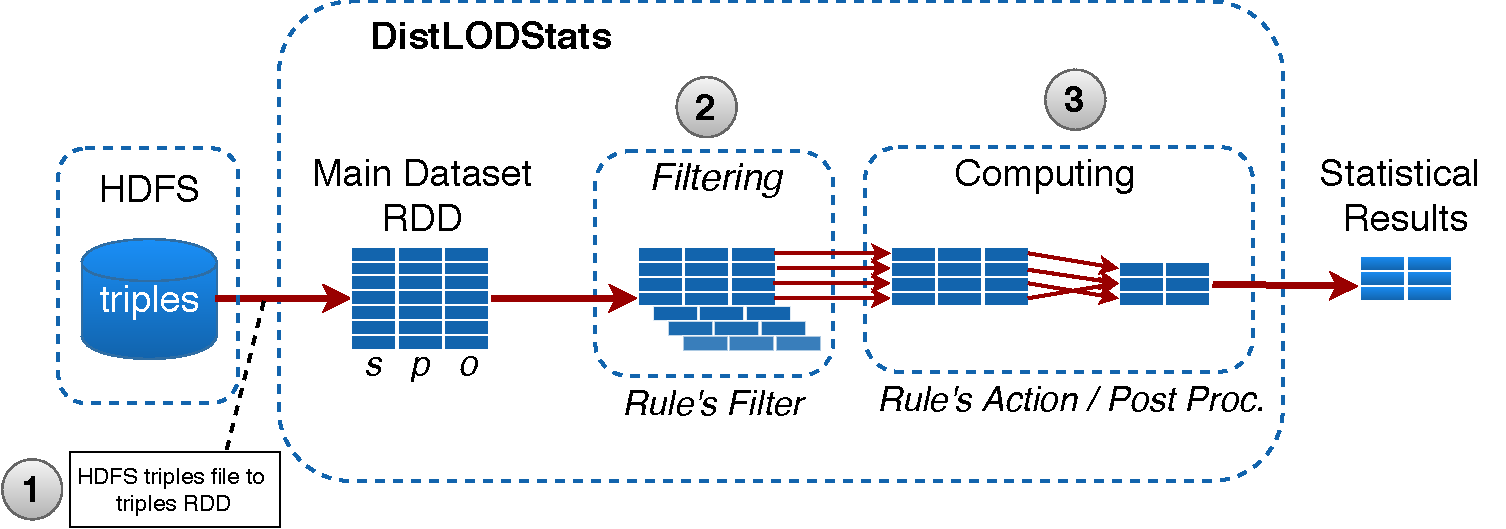
\includegraphics[width=1.0\textwidth]{images/4_distlodstats/distlodstats-system.pdf}
\caption{\textbf{Overview of DistLODStats's abstract architecture}. It is composed of three steps: First, it reads RDF data from HDFS and converts them into RDD of triples. Second, this latter undergoes a Filtering operation applying the Rule's Filter and producing a new filtered RDD. Third, the filtered RDD will serve as an input to the next step: Computing where the rule's action and/or post-processing are effectively applied. As a result, a statistical representation is generated.}
\label{fig:DistLODStatsSystem}
\end{figure*}
Furthermore, we provide a Docker image of the system\furl{https://github.com/SANSA-Stack/Spark-RDF-Statistics} available under \textit{Apache License 2.0}, integrated within the BDE platform\furl{https://github.com/big-data-europe} - an open-source Big Data Processing Platform allowing users to install numerous big data processing tools and frameworks and create working data flow applications.

We implemented DistLODStats using Spark-2.2.0, Scala 2.11.11 and Java 8. 
DistLODStats has meanwhile been integrated into SANSA~\cite{lehmann-2017-sansa-iswc,iermilov-2017-sansa-iswc-demo}, an open source\furl{https://github.com/SANSA-Stack} \emph{data flow processing engine} for performing distributed computation over large-scale \gls{RDF} datasets. 
It provides data distribution, communication, and fault tolerance for manipulating large \gls{RDF} graphs and applying machine learning algorithms on the data at scale. 
Via this integration, DistLODStats can also leverage the developer and user community as well as infrastructure behind the SANSA project. 
This also ensures the sustainability of DistLODStats given that SANSA is backed by several grants until at least 2021.


\subsection{Evaluation}
\label{sec:evaluation}
The aim of our evaluation is to see how well our approach can perform against non-distributed approaches as well as analyzing the scalability of the distributed approach. 
In particular, we addressed the following questions:   
\begin{itemize}
    \item ($Q_1$): How does the runtime of the algorithm change when more nodes in the cluster are added?
    \item ($Q_2$): How does the algorithm scale to larger datasets?
    \item ($Q_3$): How does the algorithm scale to a larger number of datasets?
\end{itemize}

In the following, we present our experimental setup including the datasets used. Thereafter, we give an overview of our results, which we subsequently discuss in the final part of this section.

\subsubsection{Experimental Setup}
We used one synthetic and two real-world datasets for our experiments:
\begin{enumerate}
 
 \item We chose the geospatial dataset LinkedGeoData~\cite{SLHA11} which offers a spatial \gls{RDF} knowledge base derived from OpenStreetMap.
 
 \item As a cross-domain dataset, we selected \emph{DBpedia}~\cite{dbpedia-swj} (v 3.9). DBpedia is a knowledge base with a large ontology.
 
 \item As a synthetic dataset, we chose to use the Berlin \gls{SPARQL} Benchmark (BSBM)~\cite{Bizer2009TheBS}.
 It is based on an e-commerce use case which is built around a set of products that are offered by different vendors.
 The benchmark provides a data generator, which can be used to create sets of connected triples of any particular size.
 
\end{enumerate}

Properties of these datasets are given in Table~\ref{tab:dataset_info}.

\begin{table*}
\centering
\begin{tabularx}{\textwidth}{Xcccccccc}	
\toprule
\multirow{2}{*}{$\longrightarrow$} & \multicolumn{1}{c}{} & \multicolumn{3}{c|}{DBpedia} & \multicolumn{3}{c}{BSBM} \\
\cline{3-9}  \rule{0pt}{10pt}
& LinkedGeoData & \scriptsize{en} & \scriptsize{de} & \scriptsize{fr}  & \scriptsize{2GB} &\scriptsize{20GB} &\scriptsize{200GB}\\
\midrule
\scriptsize{\#nr. of triples}& \scriptsize{1,292,933,812} & \scriptsize{812,545,486} & \scriptsize{336,714,883} & \scriptsize{340,849,556} & \scriptsize{8,289,484} & \scriptsize{81,980,472} & \scriptsize{817,774,057} & \\
\scriptsize{size (GB)} & \scriptsize{191.17} & \scriptsize{114.4} & \scriptsize{48.6} & \scriptsize{49.77} & \scriptsize{2} &\scriptsize{20} &\scriptsize{200} & \\
\bottomrule
\end{tabularx}
{\caption{\textbf{Dataset summary information (nt format)}.
Lists dataset characteristics used on the evaluation of the DistLODStats.
The size (in GB) and the number of triples are given.}
\label{tab:dataset_info}}
\end{table*}

For the evaluation, all data is stored on the same \gls{HDFS} cluster using Hadoop 2.8.0.
All experiments were carried out on a 6 nodes cluster (1 master, 5 workers): Intel(R) Xeon(R) CPU E5-2620 v4 @ 2.10GHz (32 Cores), 128 GB RAM, 12 TB SATA RAID-5.
The experiments on a local mode are all performed on a single instance of the cluster.
The machines were connected via a Gigabit network.
All experiments were executed three times and the average value is reported.

\subsubsection{Results}
% https://docs.google.com/spreadsheets/d/1sPdebCLTX2NK2JTvRS2TdFIPiibHWRfXT4XmBHPi0i4/edit
We evaluate our approach using the above datasets to compare it against the original LODStats.
We carried out two sets of experiments.
First, we evaluate the execution time of our distributed approach against the original approach.
Second, we evaluate the horizontal scalability via increasing nodes (machines) in the cluster. 
Results of the experiments are presented in Table~\ref{tbl:statistics}, Figure~\ref{fig:Speedup}, \ref{fig:Sizeup} and \ref{fig:Scalability}.

\defn{Distributed Processing on Large-Scale Datasets}
\label{subsubsection:large_scale_datasets}
To address $Q_1$, we started our experiments by evaluating the \textit{speedup} gained by adopting a distributed implementation of LODStats criteria using our approach, and compare it against the original centralized version.
We run the experiments on four datasets
($DBpedia_{en}$, $DBpedia_{de}$, $DBpedia_{fr}$, and $LinkedGeoData$) in a local environment on a single instance with two configurations:  (1) files of the dataset are considered separately, and (2) one big file--all files concatenated.

\begin{table*}
\centering
\begin{tabularx}{\textwidth}{Xcccccc}	
\toprule
\multicolumn{1}{l}{}& \multicolumn{5}{c}{\scriptsize{Runtime (h)} (\scriptsize{mean/std})} \\
\cline{2-6}
\rule{0pt}{8pt}
\multirow{2}{*}{$\longrightarrow$} & \multicolumn{2}{c|}{\scriptsize{\textbf{LODStats}}} & \multicolumn{3}{c}{\scriptsize{\textbf{DistLODStats}}} \\
\cline{2-6}  \rule{0pt}{10pt}
& \scriptsize{a) files} & \scriptsize{b) bigfile}  & \scriptsize{c) local} & \scriptsize{d) cluster} & \scriptsize{e) speedup ratio} \\
\midrule
\scriptsize{LinkedGeoData}& \textcolor{blue}{\scriptsize{n/a}} & \textcolor{blue}{\scriptsize{n/a}} & \scriptsize{36.65/0.13} & \win \scriptsize{4.37/0.15} & \scriptsize{7.4x}\\ \scriptsize{M$_{DBpedia}^{en}$} & \win \scriptsize{24.63/0.57} & \textcolor{red}{\scriptsize{fail}} & \scriptsize{25.34/0.11} & \win \scriptsize{2.97/0.08} & \scriptsize{7.6x} \\
\scriptsize{M$_{DBpedia}^{de}$} & \textcolor{blue}{\scriptsize{n/a}} & \textcolor{blue}{\scriptsize{n/a}} & \scriptsize{10.34/0.06} & \win \scriptsize{1.2/0.0} & \scriptsize{7.3x}\\
\scriptsize{M$_{DBpedia}^{fr}$} & \textcolor{blue}{\scriptsize{n/a}} & \textcolor{blue}{\scriptsize{n/a}} & \scriptsize{10.49/0.09} & \win \scriptsize{1.27/0.04} & \scriptsize{7.3x}\\
\bottomrule
\end{tabularx}
{\caption{\textbf{Distributed Processing on Large-Scale Datasets}.
Reports the performance analysis of the \textit{speedup} gained by DistLODStats as compared with the original centralized version.
The experiments were run on four datasets ($DBpedia_{en}$, $DBpedia_{de}$, $DBpedia_{fr}$, and $LinkedGeoData$) in a local environment on a single instance with two configurations:  (1) files of the dataset are considered separately, and (2) one big file--all files concatenated.
}
\label{tbl:statistics}}
\end{table*}

Table~\ref{tbl:statistics} shows the performance of two algorithms applied to the four datasets.
The column LODStats$^{a)}$ reports on the performance of LODStats on files separately (considering each file as a sequence of execution), the next columns LODStats$^{b)}$ reports on the performance of LODStats using a single big file by concatenating each file, and the last columns reports on the performance of DistLODStats on the same case as previously i.e. the performance for one big dataset in local mode $c)$ and cluster mode $d)$.
We observe that the execution in DistLODStats$^{c), d)}$ finishes with all the datasets (see Figure~\ref{fig:Speedup}).
However, for LODStats$^{a), b)}$ the execution often fails at different stages of the execution.
In particular, \emph{n/a} indicates parser exceptions and \emph{fail} out of memory exceptions.
The only case where the execution finishes and actually slightly outperforms DistLODStats$^{c)}$ on a single node is executing LODStats on the dataset ${DBpedia}^{en}$ split into files (25.34h for DistLODStats$^{c)}$ vs 24.63h in LODStats$^{a)}$). 
This is because the DistLODStats$^{c)}$ considers the input dataset as a big file instead of evaluation it on each file separately. 
LODStats streams the criteria one by one, so having a large dataset streamed that way would lead to very high processing times.
However, with small data as input, the processing can finish in short amount of time, but the results can be very inaccurate.

\begin{figure}
  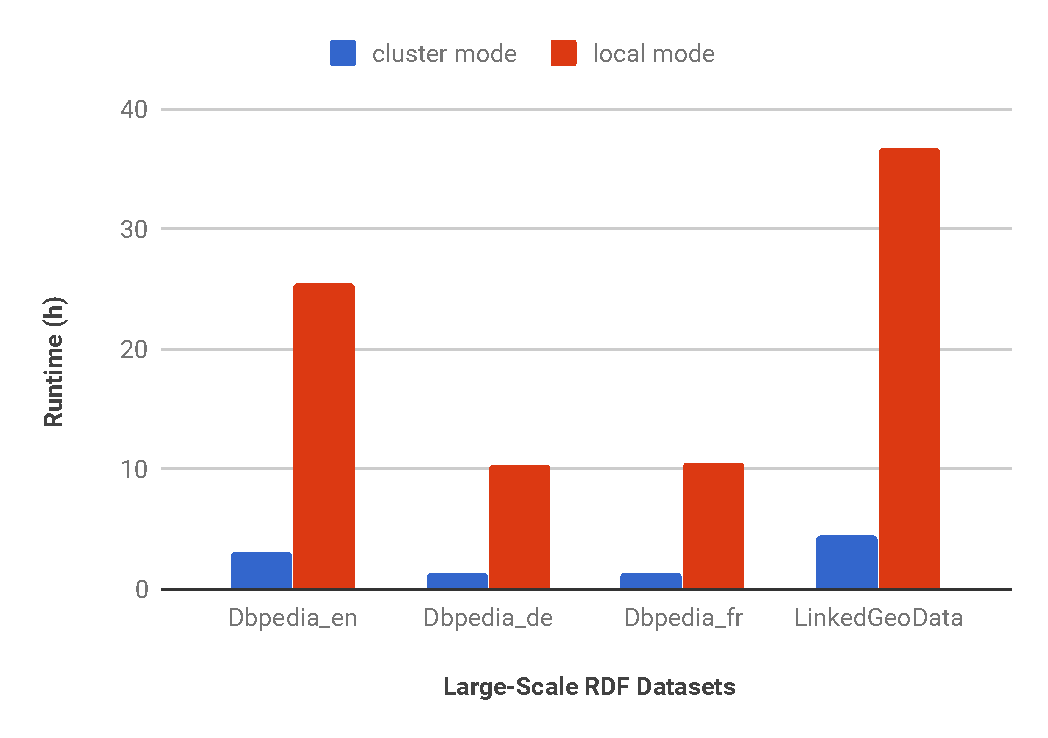
\includegraphics[width=1.0\columnwidth]{images/4_distlodstats/distlodstats-speedup-performance.pdf}
    \caption{\textbf{Speedup performance evaluation of DistLODStats}. Reports speedup performance analysis for large-scale RDF datasets for DistLODStats on local mode and cluster mode, respectively. All results illustrate consistent improvement for each dataset when running on a cluster. The geometric mean of the speedup is 7.4x.}
    \label{fig:Speedup}
\end{figure}

Figure~\ref{fig:Speedup} shows the speedup performance evaluation for large-scale \gls{RDF} datasets for DistLODStats on local mode and cluster mode, respectively.
All results illustrate consistent improvement for each dataset when running on a cluster. 
The maximum speedup is 7.6x and the geometric mean of the speedup is 7.4x.

For example, on ${DBpedia}_{en}$, the time on cluster mode is about 2.97 hours which is 7.6 times faster than evaluating DistLODStats on local mode (about 25.34 hours). 
The reason why the time spent on local mode extremely decreases is that the size of the working directory of worker processes is too large and Spark uses threads for distributing the tasks.

\defn{Scalability}
\textit{Sizeup scalability} 
To measure the performance of \textit{size-up} i.e.~scalability of our approach, we run experiments on three different sizes.
This analysis keeps the number of nodes in a cluster constant, we fix the number of workers (nodes) to 5 and grow the size of datasets to measure whether a given algorithm can deal with larger datasets.
Since real-world datasets are considered to be unique in the size and also on other aspects e.g.~number of unique terms, we chose the BSBM benchmark tool to generate artificial datasets of different sizes.
We started by generating a dataset of 2GB.
Then we iteratively increased the size of datasets by one order of magnitude.

On each dataset, we ran the distributed algorithm and the runtime is reported on Figure~\ref{fig:Sizeup}.
The $x$-axis is a generated BSBM dataset per each order of 10x magnitude.

\begin{figure}
 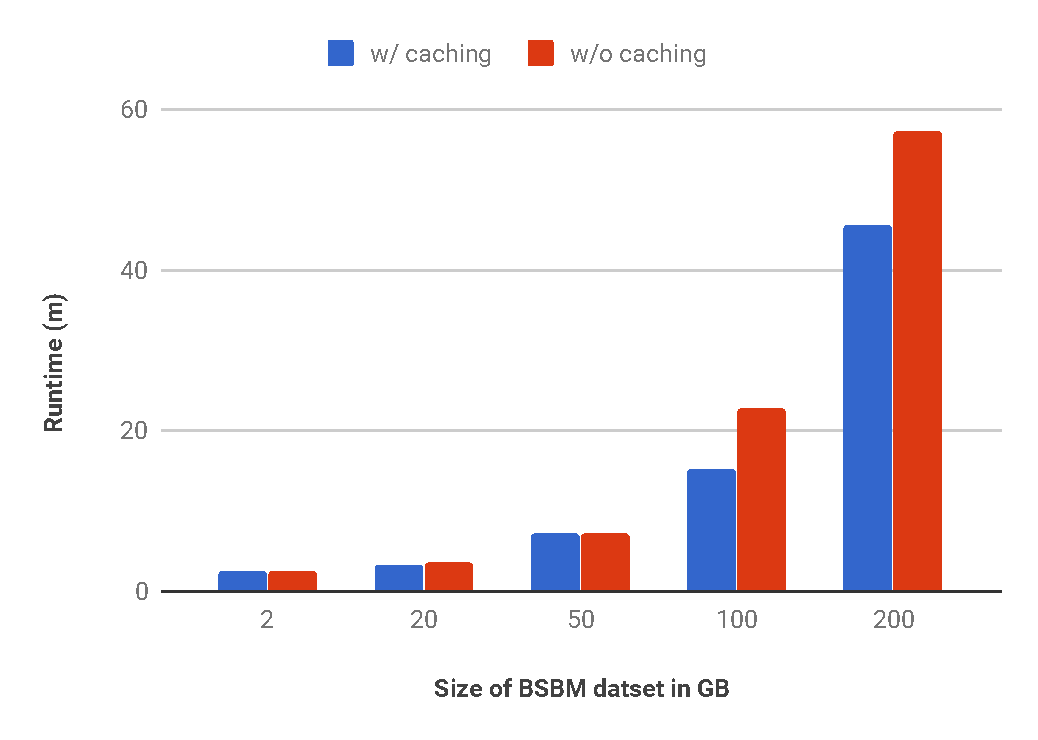
\includegraphics[width=1.0\columnwidth]{images/4_distlodstats/distlodstats-sizeup-performance.pdf}
\caption{\textbf{Sizeup performance evaluation of DistLODStats}.
The analysis keeps the number of nodes in a cluster constant (5 worker nodes) and grows the size of datasets (BSBM) to measure whether our approach can deal with larger datasets.
We see that the execution time cost grows linearly and is near-constant when the size of the dataset increases.
It stays near-constant as long as the data fits in memory which demonstrates one of the advantages of utilizing an in-memory approach in performing the statistics computation.
}
\label{fig:Sizeup}
\end{figure}

By comparing the runtime (see Figure~\ref{fig:Sizeup}), we note that the execution time cost grows linearly and is near-constant when the size of the dataset increases.
As expected, it stays near-constant as long as the data fits in memory.
This demonstrates one of the advantages of utilizing an in-memory approach in performing the statistics computation.
The overall time spent in data read/write and network communication found in disk-based approaches is no present in distributed in-memory computing. 
The performance only starts to degrade when substantial amounts of data need to be written to disk due to memory overflows. 
The results show the scalability of our algorithm in the context of sizeup, which answers question $Q_2$.

\noindent
\textit{Node scalability} In order to measure node scalability, we use variations of the number of workers on our cluster.
The number of workers varies from 1, 2, 3 and 4 to 5.

\begin{figure}
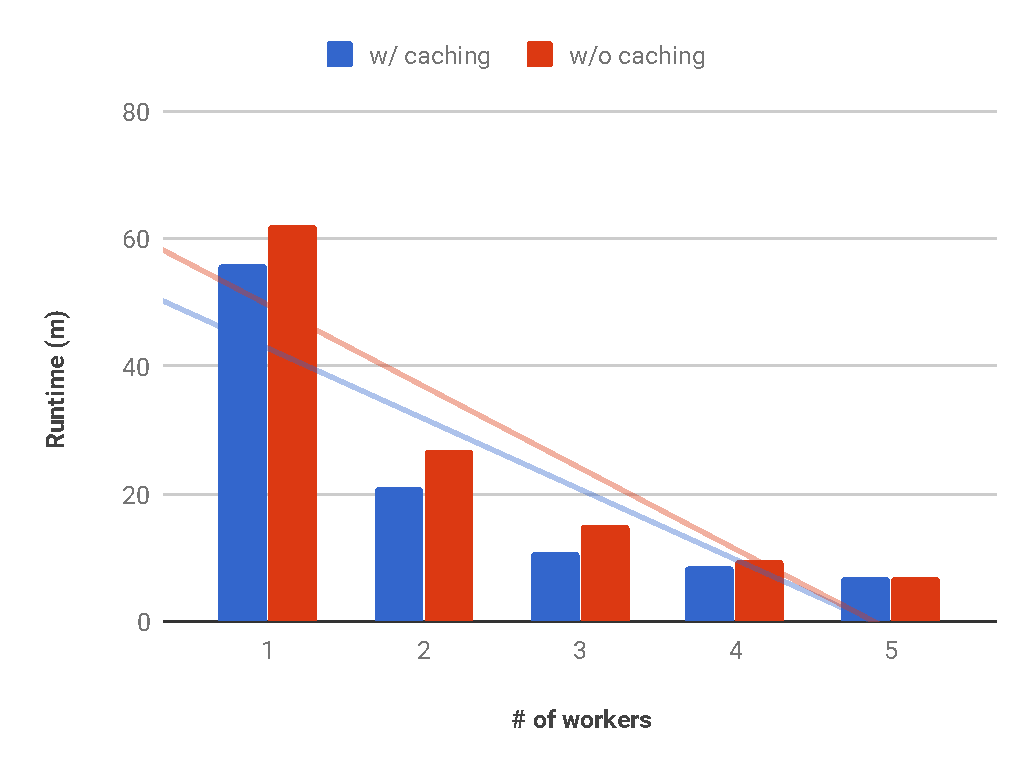
\includegraphics[width=1.0\columnwidth]{images/4_distlodstats/distlodstats-node-scalability.pdf}
\caption{\textbf{Scalability performance evaluation on DistLODStats}.
The analysis keeps the size of the dataset constant ($BSBM_{50GB}$) and varies the number of workers on the cluster.
The number of workers varies from 1, 2, 3, and 4 to 5.
We can see that as the number of workers increases, the execution time cost is super-linear on $BSBM_{50GB}$ dataset.}
\label{fig:Scalability}
\end{figure}

Let $T_N$ be the time required to complete the task on $N$ workers. The speedup $S$ is the ratio
$ S = \frac{T_L}{T_N},$
where $T_L$ is the execution time of the algorithm on local mode.
Efficiency measures the processing power being used (i.e~speedup per worker). 
It is defined as the time to run the algorithm on $N$ workers compared to the time to run algorithm on local mode:
$ E = \frac{S}{N} =\frac{T_{L}}{N T_{N}}.$

Figure~\ref{fig:Scalability} shows the speedup for $BSBM_{50GB}$.
We can see that as the number of workers increases, the execution time cost is super-linear.

As depicted in Figure~\ref{fig:Effectiveness}, the speedup performance trend is consistent as the number of workers increases.

\begin{figure}
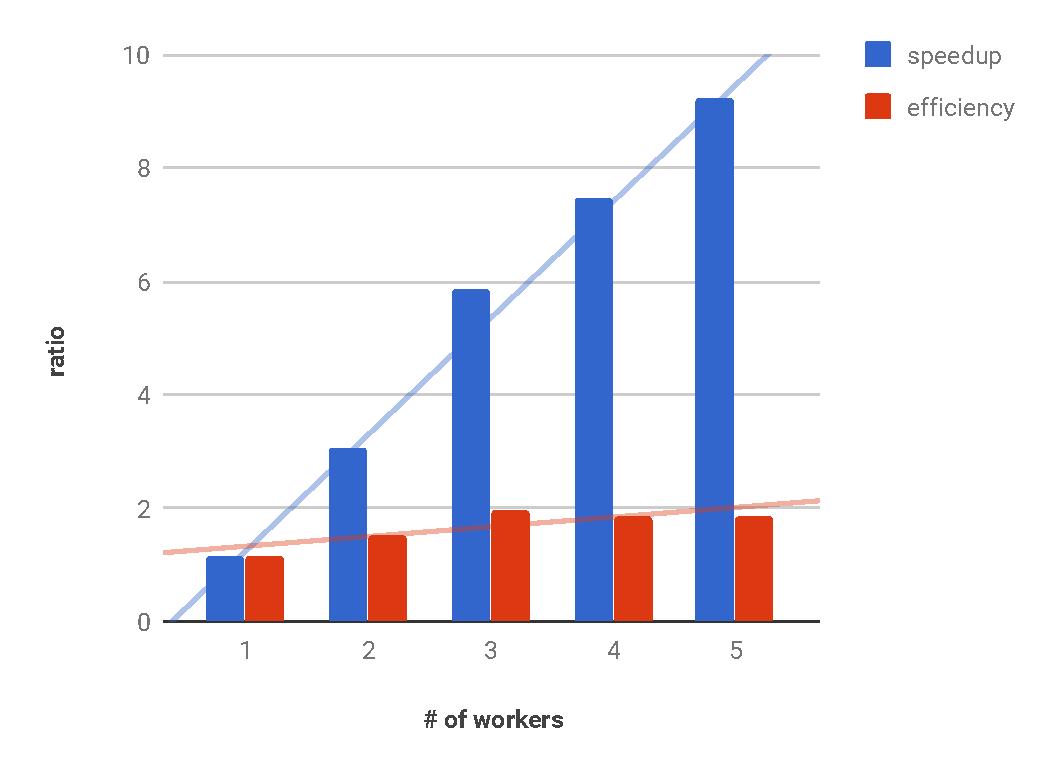
\includegraphics[width=1.0\columnwidth]{images/4_distlodstats/distlodstats-effectiveness.pdf}
\caption{\textbf{Speedup Ratio and Efficiency of DistLODStats}.
The speedup performance trend is consistent as the number of workers increases.
Efficiency increased only up to the 4th worker for $BSBM_{50GB}$ dataset.
The results imply that DistLODStats can achieve near-linear or even superlinear scalability in performance.}
\label{fig:Effectiveness}
\end{figure}

In contrast, as the number of workers was increased from 1 to 5, efficiency increased only up to the 4th worker for $BSBM_{50GB}$ dataset.
This implies that the tasks generated from the given dataset were covered with almost 4 nodes.
The results imply that DistLODStats can achieve near-linear or even superlinear scalability in performance, which answers question $Q_3$.

\defn{Breakdown by Criterion}\hspace*{\fill} \\
Now we analyze the overall runtime of criteria execution.
Figure~\ref{fig:Breakdown} reports on the runtime of each criterion on both $BSBM_{20GB}$ and $BSBM_{200GB}$ datasets.

\begin{figure*}
\centering
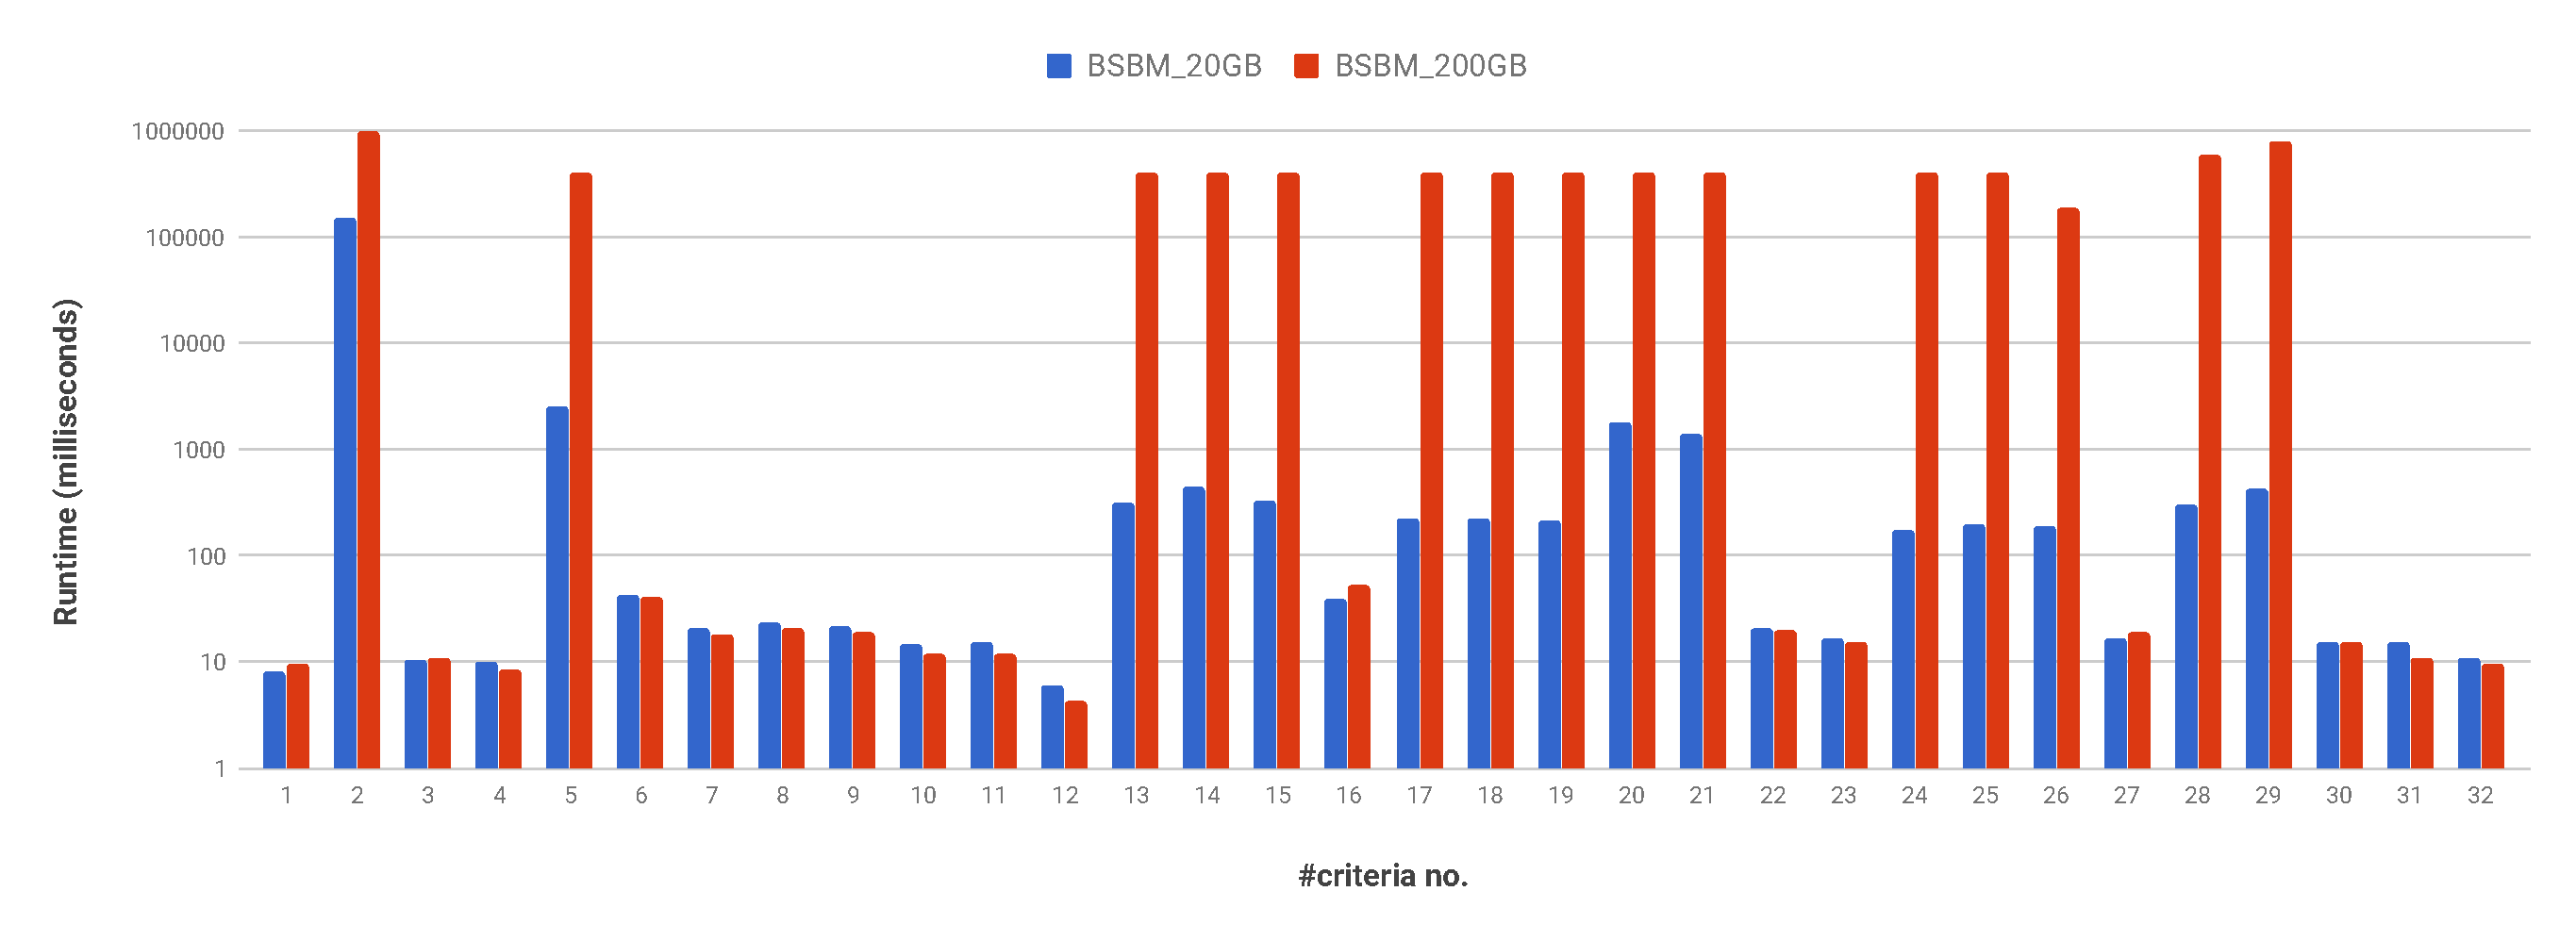
\includegraphics[width=1\columnwidth]{images/4_distlodstats/distlodstats-overall-breakdown.pdf}
\caption{\textbf{Overall Breakdown by Criterion Analysis (log scale)}.
The execution time is longer when there is data movement in the cluster compared to when data is processed without movement.
There are some criteria that are quite efficient to compute even with data movement e.g. 22, 23. 
This is because data is largely filtered before the movement.
}
\label{fig:Breakdown}
\end{figure*}

\textbf{Discussion.}
DistLODStats consists of 32 predefined criteria most of which have a runtime complexity of $O(n)$ where $n$ is the number of input triples. The breakdown for BSBM with two instances is shown in Figure~\ref{fig:Breakdown}.
The results obtained confirm to a large extent the pre-analysis made in Figure~\ref{subsection:complexAnalys}.
The execution is longer when there is data movement in the cluster compared to when data is processed without movement e.g.~Criterion \ref{cr:2}, \ref{cr:3} and \ref{cr:4}.
There are some criteria that are quite efficient to compute even with data movement e.g.~\ref{cr:22}, \ref{cr:23}. This is because data is largely filtered before the movement. 
Criterion~\ref{cr:2} and \ref{cr:28} are the most expensive ones in terms of time of execution.
This is most probably because of the sorting and maximum algorithm used by Spark.
Criteria~\ref{cr:20} and \ref{cr:21} are particularly expensive because of the extra overhead caused by extracting the data type and language for each particular object of type Literal.
Criteria like \ref{cr:14} and \ref{cr:15} do not require movement of data, but yet are inefficient in execution. This is because the data is not filtered previously.
The last three criteria do include data movement but are among the most efficient ones.
This is because the low number of namespaces the chosen datasets have.

Overall, the evaluation study conducted demonstrates that parallel and distributed computation of the different statistical values is scalable, i.e.~the execution finishes in a reasonable time relative to the high volume of datasets.


\section{STATisfy: A REST Interface for DistLODStats}
\label{sec:distlodstats-statisfy}
The increasing adoption of the Linked Data format, \gls{RDF}, over the last two decades has brought new opportunities.
It has also raised new challenges though, especially when it comes to managing and processing large amounts of \gls{RDF} data.
In particular, assessing the internal structure of a data set is important, since it enables users to understand the data better.
One prominent way of assessment is computing statistics about the instances and schema of a data set.
However, computing statistics of large \gls{RDF} data is computationally expensive.
To overcome this challenging situation, we previously built DistLODStats, a framework for parallel calculation of 32 statistical criteria over large \gls{RDF} datasets, based on Apache Spark.
Running DistLODStats is, thus, done via submitting jobs to a Spark cluster.
Often times, this process is done manually, either by connecting to the cluster machine or via a dedicated resource manager. 

SANSA and DistLODStats use Apache Spark\furl{http://spark.apache.org/} as an underlying engine, which is a popular framework for processing large datasets in-memory.
Spark provides two possibilities of running and interacting with applications: 
\begin{itemize}
    \item \textit{Interactive} - via a \gls{CLI} called \textit{Spark Shell}, or via Spark \textit{Notebooks} (e.g. SANSA-Notebooks~\cite{iermilov-2017-sansa-iswc-demo}),
    \item \textit{Batch} - which includes a bash script called \textit{spark-submit} used to submit a Spark application to the cluster without interaction during run time.
\end{itemize}

Spark application is usually launched by logging first into a cluster, either in the premises or remotely in the cloud. This process presents several difficulties:
\begin{itemize}
    \item It requires a sophisticated user access control management, which may become hard to maintain with multiple users.
    \item It raises the chances of exhausting the cluster or even causing its failure.
    \item It exposes cluster and its configurations to all the users with access.
\end{itemize}

In order to elevate those, we have investigated Apache Livy~\furl{https://livy.incubator.apache.org/} -- a novel open-source REST interface for interacting remotely with Apache Spark. It supports executing snippets of code or programs in a Spark context that runs locally, in a Spark cluster or in Apache Hadoop YARN.

\subsection{System Design Overview}
Traditionally, when running a Spark job, submitting it to a Spark cluster is done via a \textit{spark-shell} or \textit{spark-submit}.
Usually, this process is done manually either entering the cluster gateway machines or via a dedicated resource manager (e.g. SLURM, OpenStack). 

\begin{figure*}
\centering
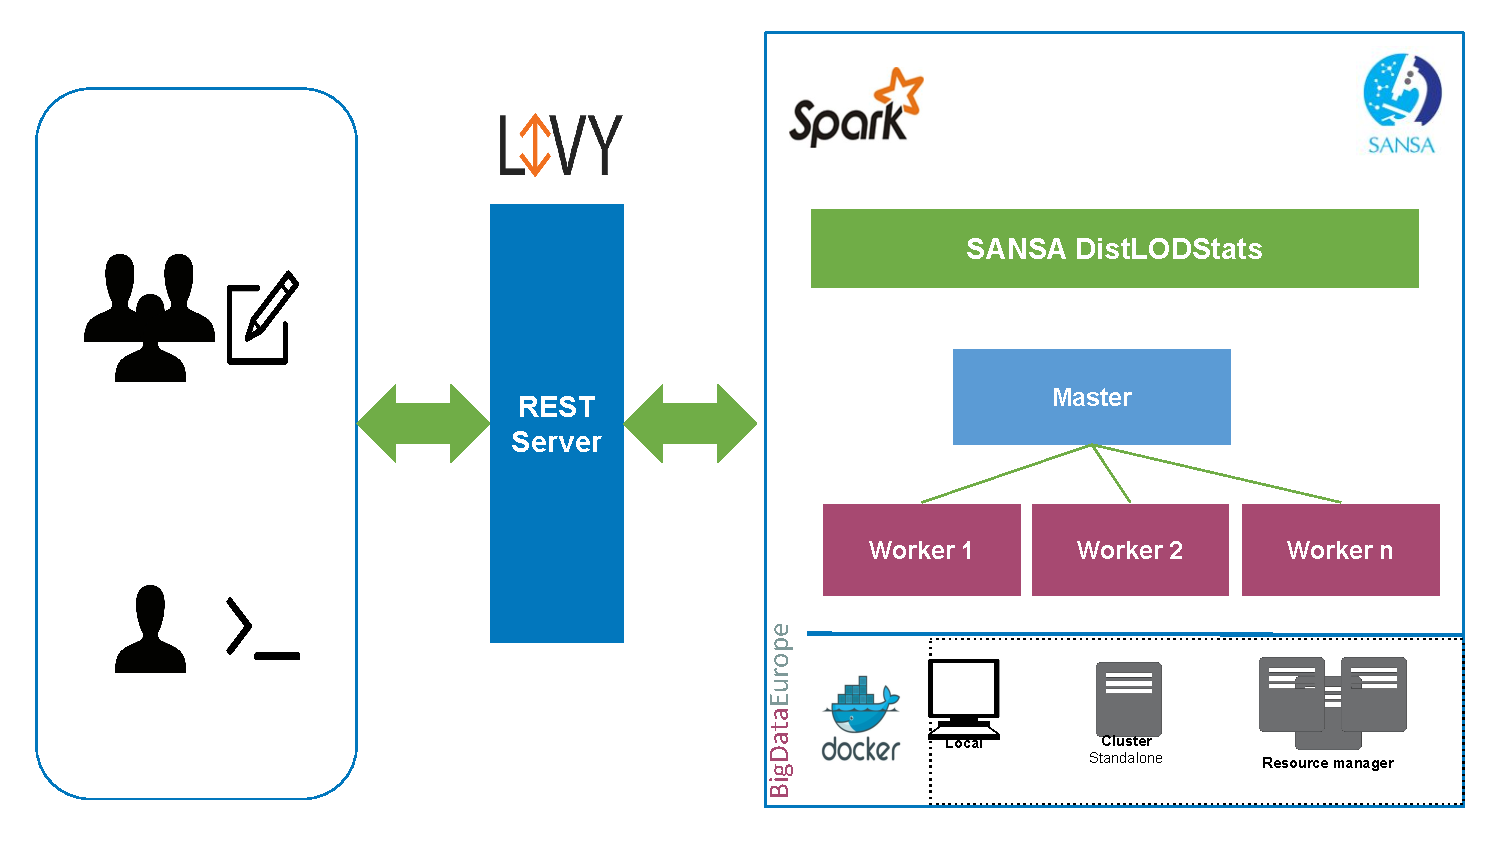
\includegraphics[width=1.0\columnwidth]{images/4_distlodstats/distlodstats-statisfy.pdf}
\caption{\textbf{STATisfy overview architecture}.
Main services of STATisfy: \textit{Client} -- will create a remote Spark cluster for initialization, and submit jobs through REST APIs.
\textit{Livy REST Server} -- it will then discover this job and sent through Remote Procedure Call (RCP) to SparkSession, where the code will be initialized and executed using DistLODStats.
}
\label{fig:STATisfy}
%source:https://docs.google.com/presentation/d/1bV83Rik_xwzmYPigCwHWV9OMQC5Wtl3gSF4UoaNilIQ
\end{figure*}

For users with little experience in cluster management and the Hadoop infrastructure, it can be challenging to run Spark.
As an alternative, we introduce \textbf{STATisfy}\furl{https://github.com/GezimSejdiu/STATisfy}: REST Interface for DistLODStats. 

Instead of computing \gls{RDF} statistics directly on the cluster, the interaction is done via REST APIs (as it is depicted in the Figure~\ref{fig:STATisfy}).

The client-side will create a remote Spark cluster for initialization, and submit jobs through REST APIs. 
Livy REST Server will then discover this job and send it through \gls{RCP} to SparkSession, where the code will be initialized and executed.
In the meantime, the client will be waiting for the result of this job coming from the same direction.

Running the STATisfy is similar to using DistLODStats via \textit{spark-submit}.
The difference is that this shell is not running locally, instead, it runs in a cluster and transfers the data back and forth through the network.

For demonstrating the usage of the tool, we have deployed it on the comprehensive statistics catalog LODStats\furl{http://lodstats.aksw.org/} which crawls \gls{RDF} data from metadata portals such as CKAN dataset metadata registry. 
By doing this, it obtains a comprehensive picture of the current state of the Web of Data.
As we use DistLODStats as an underlying engine for computing \gls{RDF} statistics afterward, the limitation was that the user has to interact with the cluster manually and initiate the job for computing such statistics.
By using STATisfy REST interface, LODStats will interact with the cluster from anywhere which provides the capabilities necessary to do this without compromising on ease of use or security.

As it is shown in Figure~\ref{fig:STATisfy}, the user starts a session via REST \gls{API} using Livy for submitting a job to the Spark cluster.
With the POST request, the user could submit a request to DistLODStats using the Livy server. 
Using Livy, STATisfy will then help to launch this request in the cluster.
As a result, the output will be curled by their end in the format of the VoID description.


\section{Summary}
\label{sec:distlodstats-summary}
For obtaining an overview over the Web of Data as well as evaluating the quality of individual datasets, it is important to gather statistical information describing characteristics of the internal structure of datasets.
However, this process is both data-intensive and computing-intensive and it is a challenge to develop fast and efficient algorithms that can handle large scale \gls{RDF} datasets.

In this chapter, we presented DistLODStats, a novel software component for distributed in-memory computation of \gls{RDF} datasets statistics implemented using the Spark framework.
DistLODStats is maintained and has an active community due to its integration in SANSA. 
Our definition of statistical criteria provides a framework reducing the implementation effort required for adding further statistical criteria. 
We showed that our approach improves upon a previous centralized approach we compare against.
Since Spark \gls{RDD}s are designed to scale horizontally, cluster sizes can be adapted to dataset sizes accordingly. 

DistLODStats is a prominent solution, however, it requires setup and managing of the cluster configuration and job submission.
To make the process easier, we have introduced STATisfy, a tool for interacting with DistLODStats via a REST Interface.
This way DistLODStats can be provided as-a-service, where users only send (HTTP) requests to the remote cluster and obtain the wished results, without having any knowledge about system access or cluster management.
STATisfy is used for the LODStats project and inclusion in the new DBpedia\furl{https://wiki.dbpedia.org/} community release processes is ongoing.